\documentclass{beamer}
\usetheme{Berlin} % Warsaw como modelo não estava funcionando bem, apesar de ficar MUITO BOM, Berlin ficou mais claro
\usepackage[utf8]{inputenc}
\usepackage[T1]{fontenc}
\usepackage{graphicx}
\usepackage{tikz}
\usepackage{booktabs}
\usepackage{listings}
\usepackage{hyperref} % Hyperlinks estavam dando problema antes
% Para definir o estilo de codigo para os exemplos de pascal

\lstset{
    language=Pascal,
    basicstyle=\footnotesize\ttfamily,
    keywordstyle=\color{blue},
    commentstyle=\color{green},
    stringstyle=\color{red},
    breaklines=true,
    frame=single
}

% Informação da pagina de titulo, tive que mudar a escala para 0.45 no logo, estava dando errado com 0.6
\title{Linguagem de Programação: Grupo 1 - Pascal}
\subtitle{Trabalho Teórico Prático (TTP) - Disciplina: Linguagens de Programação}
\author{Edgard de Paiva Melo Filho, Maicon Gomes Mesias}
\institute{\includegraphics[scale=0.45]{LOGO_PUC.png}\\Pontifícia Universidade Católica de Minas Gerais \\ Instituto de Ciências Exatas e Informática \\ Curso de Engenharia de Computação}
\date{16 de Setembro de 2025}
\begin{document}
% Capa (Title Slide)
\frame{\titlepage}
% Sumário / Roteiro / Agenda
\begin{frame}{Sumário / Roteiro / Agenda}
\tableofcontents
\end{frame}
\section{Introdução}
\begin{frame}{Introdução}
\begin{itemize}
\item A linguagem de programação Pascal surgiu em 1970, criada por Niklaus Wirth na Universidade Federal de Zurique (ETH Zurich), com o objetivo de oferecer uma linguagem estruturada, clara e eficiente para o ensino da programação e da ciência da computação.
\item Importância: Adotada amplamente em universidades e escolas técnicas durante as décadas de 1970, 1980 e início de 1990; introduziu conceitos fundamentais de programação estruturada que influenciaram linguagens modernas como Python, Java e C++ direta ou indiretamenta.
\end{itemize}
\end{frame}

\section{Linha do Tempo & Genealogia da Linguagem}
\begin{frame}{Linha do Tempo}
    \begin{figure}[H]
    \centering
    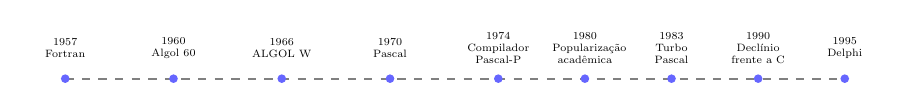
\begin{tikzpicture}[>=stealth, scale=0.55, transform shape]
        \draw[thick, gray, dashed] (0,0) -- (18,0);
        \foreach \x/\ano/\evento in {
            0/1957/Fortran,
            2.5/1960/Algol 60,
            5/1966/ALGOL W,
            7.5/1970/Pascal,
            10/1974/Compilador Pascal-P,
            12/1980/Popularização acadêmica,
            14/1983/Turbo Pascal,
            16/1990/Declínio frente a C/C++,
            18/1995/Delphi/Object Pascal
        }{
            \node[circle, fill=blue!60, inner sep=2pt] at (\x,0) {};
            \node[align=center, font=\scriptsize, text width=1.5cm] at (\x,0.7) {\ano \\ \evento};
        }
    \end{tikzpicture}
    \caption{Linha do tempo da evolução da linguagem Pascal}
    \label{fig:cronologia-pascal}
    \end{figure}
\end{frame}

\begin{frame}{Linha do Tempo}
    \includegraphics[scale=0.35]{linhaDoTempo.jpeg}
\end{frame}

\begin{frame}{Genealogia da Linguagem}
    \centering
    \includegraphics[scale=0.4]{Genealogia.jpeg}
\end{frame}

\section{Paradigma(s) a que Pertence (Características Principais)}
\begin{frame}{Paradigmas e Características Principais}
\begin{itemize}
\item \textbf{Paradigma Imperativo}: O programa é descrito como uma sequência de comandos que alteram o estado do computador, tendo instruções claras de 'o que fazer' e 'como fazer'.
\item \textbf{Paradigma Procedural}: Código organizado em procedimentos e funções para modularização e reutilização (ex.: procedure ExibirMensagem; begin writeln('Olá, mundo!'); end;).
\item \textbf{Paradigma Estruturado}: Ênfase em blocos (begin...end), estruturas de controle (IF...THEN...ELSE, FOR, WHILE) e fluxo lógico claro, evitando goto excessivo.
\item Ênfase em legibilidade, ensino e organização lógica do código.
\end{itemize}
\end{frame}
\section{Características mais Marcantes da Linguagem}
\begin{frame}{Características Marcantes}
\begin{itemize}
\item Tipagem forte e estática: Variáveis devem ter tipo definido; previne erros em tempo de compilação.
\item Tipos de dados: Integer, Real, Char, String, Boolean, Array, Record, Set, File.
\item Palavras reservadas: and, begin, case, const, do, else, end, if, of, procedure, program, repeat, then, until, var, while, etc.
\item Operadores: Aritméticos (+, -, *, /, div, mod); Relacionais (=, <>, <, >, <=, >=).
\item Estruturas de controle claras (if, while, for); suporte a procedimentos/funções aninhadas.
\end{itemize}
\end{frame}

\begin{frame}{Características Marcantes (Cont. - Resumo Visual)}
\begin{table}
\footnotesize % Para compactar e reduzir a fonte, já que estava dando spill e saindo da tabela
\begin{tabular}{p{3cm}p{6cm}}
\toprule
\textbf{Característica} & \textbf{Descrição} \\
\midrule
Fortemente Tipada & Garante tipos definidos, prevenindo erros entre tipos incompatíveis. \\
Estruturada & Blocos begin...end e fluxo lógico claro, evitando goto. \\
Procedural & Organização em procedimentos/funções para modularidade. \\
Legibilidade & Sintaxe próxima à linguagem natural (if, for, while). \\
Segurança & Tipagem forte detecta erros em compilação. \\
Suporte a Dados & Arrays, records, sets, files para organização eficiente. \\
Facilidade de Ensino & Didática para algoritmos e lógica. \\
Portabilidade & Compiladores para múltiplas plataformas. \\
\bottomrule
\end{tabular}
\end{table}
\end{frame}

\begin{frame}{Caracteristicas Marcantes - com Exemplos}
    \centering
    \includegraphics[scale=0.35]{Caracteristicas.jpeg}
\end{frame}

\section{Linguagens Relacionadas (Influenciadores, Influenciadas, Similares, “Opostas”, etc.)}
\begin{frame}{Linguagens Relacionadas}
\begin{itemize}
\item \textbf{Influenciadores}: ALGOL 60 (sintaxe e estruturas), Fortran (arrays), PL/I (modularidade).
\item \textbf{Influenciadas}: Modula-2 (1978, evolução por Wirth), Oberon (1986), Ada (1983, tipagem forte), Delphi/Object Pascal (1995).
\item \textbf{Similares}: C/C++ (estruturada e procedural, mas C menos rígido em tipagem).
\item \textbf{“Opostas”}: Linguagens dinâmicas como Python ou JavaScript (tipagem dinâmica, menos estrutura rígida).
\end{itemize}
\end{frame}

\begin{frame}{Linguagens Relacionadas - Visual}
    \centering
    \includegraphics[scale=0.35]{LinguagensRelacionadas.jpeg}
\end{frame}

\section{Exemplo(s) de Programa(s)}
\begin{frame}[fragile]{Exemplo 1: Cálculo da Média}
    \footnotesize
    \begin{lstlisting}
    program CalcMedia;
    var
      num1, num2, num3, media: real;
    begin
      writeln('Digite três números:');
      readln(num1, num2, num3);
      media := (num1 + num2 + num3) / 3;
      writeln('A média é: ', media:0:2);
    end.
    \end{lstlisting}
    \vfill
    \textbf{Descrição}: Cálculo da média de três números inseridos pelo usuário.
\end{frame}

\begin{frame}[fragile]{Exemplo 2: FizzBuzz}
    \footnotesize
    \begin{lstlisting}
    program FizzBuzz;
    var
      i: integer;
    begin
      for i := 1 to 20 do
      begin
        if (i mod 3 = 0) and (i mod 5 = 0) then
          writeln('FizzBuzz')
        else if i mod 3 = 0 then
          writeln('Fizz')
        else if i mod 5 = 0 then
          writeln('Buzz')
        else
          writeln(i);
      end;
    end.
\end{lstlisting}
\textbf{Descrição}: Imprime números de 1 a 20, substituindo múltiplos de 3 por "Fizz", de 5 por "Buzz" e de ambos por "FizzBuzz".
\end{frame}

\section{PRÁTICA: Tutoriais de Instalação, Uso e Programação + Exemplos}
\begin{frame}{Prática: Tutoriais e Exemplos}
\begin{enumerate}
\item \textbf{Instalação}: Baixe o Free Pascal Compiler (FPC) de \url{https://www.freepascal.org/}. Para Windows/Linux/macOS, siga o instalador; Lazarus IDE recomendada para desenvolvimento gráfico.
\item \textbf{Uso}: Crie arquivo .pas, compile com \texttt{fpc programa.pas}, execute o binário (./programa ou programa.exe).
\item \textbf{Exemplo prático}: Verificar se número é par ou ímpar.
\item \textbr{Opção Alternativa}: Utilize uma IDE online como por exemplo https://www.onlinegdb.com/online\_pascal\_compiler
\end{enumerate}
\end{frame}
\begin{frame}[fragile]{Exemplo Prático: Par ou Ímpar}
\begin{lstlisting}
program ParImpar;
    var numero: integer;
begin
    writeln('Digite um numero:');
    readln(numero);
    if numero mod 2 = 0 then
        writeln('Numero par')
    else
        writeln('Numero ímpar');
    readln;
end.
\end{lstlisting}
Compile e execute para testar.
\end{frame}
\section{Considerações Finais}
\begin{frame}{Considerações Finais}
\begin{itemize}
\item Legado de Pascal: Importância histórica e pedagógica; moldou gerações de programadores com conceitos de programação estruturada e tipagem forte.
\item Vantagens: Clareza, segurança, facilidade de ensino; influenciou linguagens modernas.
\item Limitações atuais: Menos usada em desenvolvimento moderno devido a linguagens mais versáteis, mas persiste em educação e legados.
\item Perspectivas futuras: Manutenção via Free Pascal; relevância em ensino de fundamentos.
\end{itemize}
\end{frame}
\section{Bibliografia}
\begin{frame}{Bibliografia}
\begin{itemize}
\item EVARISTO, Jaime. \textit{Programando com Pascal: a linguagem do Turbo Pascal e do Delphi}. 2. ed. revista. São Paulo: E-Book Express, 2000.
\item JENSEN, Kathleen; WIRTH, Niklaus. \textit{Pascal user manual and report}. 4. ed. Revisão de Andrew B. Mickel; James F. Miner. Berlin: Springer-Verlag, 1974.
\item Documentação Free Pascal: \url{https://www.freepascal.org/docs.html}.
\end{itemize}
\end{frame}
\section{Apêndice}
\begin{frame}{Apêndice: Manifestação Individual}
\textbf{Edgard de Paiva Melo Filho:} Foi com consideravel surpresa que durante a pesquisa foi visto que as primeiras versões de programas relativamente recentes em comparação com a idade da linguagem de programação, foram feitos utilizando variações de Pascal, por exemplo o Skype, onde o cliente desktop inicial foi rapidamente prototipado usando Object Pascal no ambiente de desenvolvimento Delphi.
\\
\textbf{Maicon Gomes Mesias:} Sinceramente, eu vejo o Pascal como uma linguagem que marcou época. Ela pode parecer "antiga" hoje em dia, mas teve um papel muito importante: ajudou muita gente a aprender lógica de programação de forma organizada. O legal do Pascal é que ele é bem estruturado, então não dá pra sair escrevendo código bagunçado; ele praticamente "obriga" a programar com disciplina.
\end{frame}

\end{document}
